\documentclass[preview]{standalone}

\usepackage{amsmath}
\usepackage{amssymb}
\usepackage{stellar}
\usepackage{xfrac}
\usepackage{definitions}
\usepackage{wrapfig}
\usepackage{tikz}
\usepackage{pgfplots}
\usepackage{bettelini}

\pgfplotsset{compat=1.18}

\begin{document}

\id{diffeq-exercises-qualitative}
\genpage

\section{Exercises}

\begin{snippetexercise}{diffeq-ex-22}{}
    Determine the general integral of the differential equation
    \[
        y' = -\frac{2xy + y^2 + 1}{x^2 + 2xy}
    \]
\end{snippetexercise}

\begin{snippetsolution}{diffeq-ex-22-sol}{}
    \todo
\end{snippetsolution}

\begin{snippetexercise}{diffeq-ex-23}{}
    Determine the general integral of the differential equation
    \[
        y' = \frac{y}{y^3 - x}
    \]
\end{snippetexercise}

\begin{snippetsolution}{diffeq-ex-23-sol}{}
    \todo
\end{snippetsolution}

\begin{snippetexercise}{diffeq-ex-24}{}
    Consider the following Cauchy problema
    \[
        \begin{cases}
            y' = 8x^3 (y + y^{\sfrac12}) \\
            y\left(3^{\sfrac14}\right) = 4
        \end{cases}
    \]
    \begin{enumerate}
        \item determine the local solution to the problem, indicating the biggest
        interval on which the found solution is unique;
        \item determina all the solutions of the problem on \(\realnumbers\).
    \end{enumerate}
\end{snippetexercise}

\begin{snippetsolution}{diffeq-ex-24-sol}{}
    \todo
\end{snippetsolution}

\begin{snippetexercise}{diffeq-ex-25}{}
    Consider the following differential equation
    \[
        y' = x\sin^2(y)
    \]
    \begin{enumerate}
        \item show that all the maximal solutions are defined on \(\realnumbers\), are bounded and are even functions;
        \item sketch a qualitative graph of the maximal solution to the differential equation with the initial condition \(y(0)=-1\);
        \item determine whether the solution to the previous point is integrable (in the generalized sense) on \(\realnumbers\).
    \end{enumerate}
\end{snippetexercise}

\begin{snippetsolution}{diffeq-ex-25-sol}{}
    \begin{wrapfigure}{r}{6cm}
        \begin{center}
            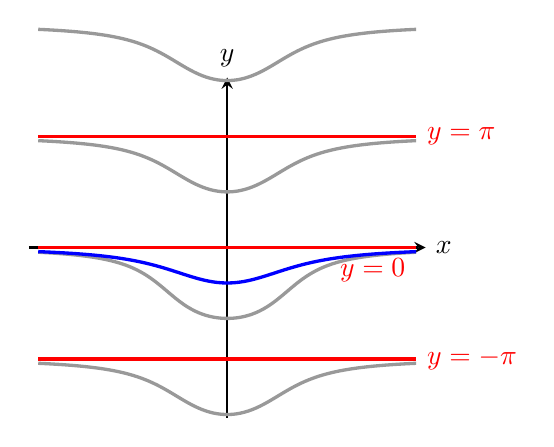
\begin{tikzpicture}[
                >=stealth,
                scale=0.5,
                x=1.2cm,
                y=0.9cm,
                declare function={
                    curve_top(\x) = rad(270 - atan(-0.5*\x*\x));
                    curve_mid(\x) = rad(90 - atan(-0.5*\x*\x));
                    blue_curve(\x) = rad(-90 - atan(-0.64209 - 0.5*\x*\x));
                    curve_deep(\x) = rad(-90 - atan(0.45766 - 0.5*\x*\x));
                    curve_bot(\x) = rad(-270 - atan(-0.5*\x*\x));
                }
            ]

            \draw[->, thick] (-4.2, 0) -- (4.2, 0) node[right] {$x$};
            \draw[->, thick] (0, -4.8) -- (0, 4.8) node[above] {$y$};

            \draw[very thick, red] (-4, -pi) -- (4, -pi) node[right] {$y=-\pi$};
            \draw[very thick, red] (-4, 0) -- (4, 0) node[below left] {$y=0$};
            \draw[very thick, red] (-4, pi) -- (4, pi) node[right] {$y=\pi$};

            \draw[very thick, gray!80, samples=100, domain=-4:4] plot (\x, {curve_top(\x)});
            \draw[very thick, gray!80, samples=100, domain=-4:4] plot (\x, {curve_mid(\x)});
            \draw[very thick, gray!80, samples=100, domain=-4:4] plot (\x, {curve_deep(\x)});
            \draw[very thick, gray!80, samples=100, domain=-4:4] plot (\x, {curve_bot(\x)});

            \draw[very thick, blue, samples=100, domain=-4:4] plot (\x, {blue_curve(\x)});

            \end{tikzpicture}
        \end{center}
    \end{wrapfigure}
    Sia \(f(x,y) = x\sin^2(y)\).
    We have local existence and uniqueness because \(f(x,y)\) is Lipschitz with respect to \(y\).
    Since
    \[
        |f(x,y)| = |x\sin^2(y)| \leq |x|\cdot |y| = \beta(x) + \alpha(x)|y|
    \]
    the solution can be extended over all \(\realnumbers\).
    The solutions are even functions because \(f(-x, y) = -f(x,y)\).
    The constant solutions are \(y=k\pi\) with \(k\) integer.
    If \(x \geq 0\), then \(y'\geq 0\) and thus the solutions are increasing to the right,
    while decreasing to the left for \(x < 0\).
    The second derivative is given by
    \[
        y'' = \sin^2(y) + 2x\sin(y)\cos(y)\cdot y'
    \]
    and at the initial point \(0\) it is strictly positive.
    The function must grow but cannot intersect the constant solution.
    So we need to study the value of this horizontal asymptote (only to the right since it is even).
    We study it in integral form for \(x \to \infty\)
    \begin{align*}
        \integral[-1][y(x)][\frac{1}{\sin^2(t)}][t] = \integral[0][x][t][t] = \frac{x^2}{x} \to \infty
    \end{align*}
    Let \(L\geq -1\) be the height of our asymptote.
    We then need to solve
    \[
        \integral[-1][L][\frac{1}{\sin^2(t)}][t] = \infty
    \]
    so this diverges for \(L=0\).
    In general, we check if the solution is integrable over all \(\realnumbers\). We have
    \begin{align*}
        \integral[-1][y(x)][\frac{1}{\sin^2(t)}][t] = \frac{x^2}{2}
    \end{align*}
    For \(x \geq 0\) we study the asymptotic
    \begin{align*}
        x &= \sqrt{
            2 \integral[-1][y(x)][\frac{1}{\sin^2(t)}][t]
        } \sim % asymptotic todo
        \underbrace{
            \sqrt{
                2\left(
                    -\frac{1}{y(x)} - 1
                \right)
            }
        }_{\geq 0}
    \end{align*}
    Hence
    \[
        2\left(-\frac{1}{y(x)} - 1\right)\sim x^2
    \]
    from which we deduce that our function behaves as
    \[
        \varphi(x) \sim - \frac{2}{x^2 + 2}
    \]
    \wrapfill
\end{snippetsolution}

\begin{snippetexercise}{diffeq-ex-26}{}
    Let \(\alpha, \beta \in \realnumbers\). Consider the Cauchy problem
    \[
        \begin{cases}
            y' = f_\alpha(y) \\
            y(0) = \beta
        \end{cases} \tag{\(P_{\alpha, \beta}\)}
    \]
    where
    \[
        f_\alpha(y) = \begin{cases}
            0 & |y| \geq 5 \\
            (25 - y^2)^{\alpha} & |y| < 5
        \end{cases}
    \]
    \begin{enumerate}
        \item Show that \((P_{\sfrac14,2})\) admits a unique solution on \(\realnumbers\),
        study this solution and sketch a qualitative graph that also takes into account the concavity.
        \item As \(\alpha,\beta\) vary study existance and uniqueness of the local solution to \((P_{\alpha,\beta})\).
        \item Determine the explicit solution to \((P_{1,0})\).
    \end{enumerate}
\end{snippetexercise}

\begin{snippetsolution}{diffeq-ex-26-sol}{}
    \todo
\end{snippetsolution}

\begin{snippetexercise}{diffeq-ex-27}{}
    Consider the differential equation
    \[
        y' = y^8 - 1. \tag{\(\ast\)}
    \]
    Show that, for any initial datum in \(\realnumbers^2\),
    there exists a unique local solution to (\(\ast\)).
    As the real parameter \(\alpha\) varies, consider the Cauchy problem
    \[
        \begin{cases}
            (\ast) \\
            y(0) = \alpha
        \end{cases}
    \]
    and let \(\varphi_\alpha\) be its maximal solution.
    For which values of \(\alpha\) is the function \(\varphi_\alpha\) constant?
    Sketch a qualitative graph of \(\varphi_\alpha\) in the three cases \(\alpha = -2\), \(\alpha = 0\), \(\alpha = 2\),
    specifying in particular the domain of definition, the lower and upper bounds, and the concavity of \(\varphi_\alpha\).
    Finally, letting \((a,b)\) be the interval of definition of \(\varphi_2\),
    determine whether there exists a left neighborhood of \(b\) on which \(\varphi_2\) is integrable (in the improper sense).
\end{snippetexercise}

\begin{snippetsolution}{diffeq-ex-27-sol}{}
    \begin{wrapfigure}{r}{6cm}
        \begin{center}
            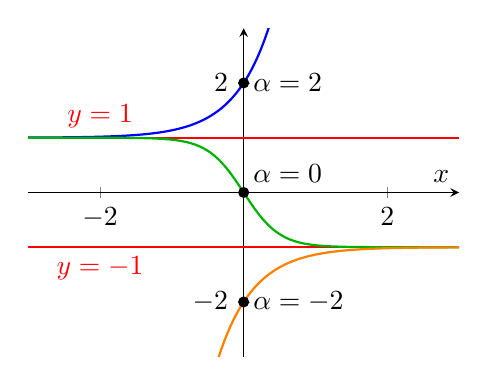
\begin{tikzpicture}
                \begin{axis}[
                    width=10cm,
                    scale=0.65,
                    height=8cm,
                    xmin=-3, xmax=3,
                    ymin=-3, ymax=3,
                    axis lines=middle,
                    xlabel=$x$,
                    %ylabel=$y$,
                    samples=100,
                    clip=true
                ]

                \addplot[red, thick, domain=-3:3] {1};
                \addplot[red, thick, domain=-3:3] {-1};

                \addplot[blue, thick, domain=-3:1] {1 + exp(2*x)};

                \addplot[green!70!black, thick, domain=-3:3] {-tanh(2*x)};

                \addplot[orange, thick, domain=-1:3] {-1 - exp(-2*x)};

                \fill[black] (axis cs:0, 2) circle (2pt) node[right] {$\alpha=2$};
                \fill[black] (axis cs:0, 0) circle (2pt) node[above right] {$\alpha=0$};
                \fill[black] (axis cs:0, -2) circle (2pt) node[right] {$\alpha=-2$};

                \node[red, above] at (axis cs:-2, 1) {$y=1$};
                \node[red, below] at (axis cs:-2, -1) {$y=-1$};

                \end{axis}
            \end{tikzpicture}
            \vspace{-1cm}
        \end{center}
    \end{wrapfigure}
    The constant solutions are \(y = \pm 1\).
    The derivative is non-negative if and only if \(|y|\geq 1\),
    therefore the solutions are increasing in the lower and upper bands.
    In the central band the solution is decreasing for \(y>0\) and decreasing for \(y \leq 0\).
    The second derivative is given by \(y'' = 8y^7y'\).
    We know that \(\varphi_0\) is bounded because it cannot intersect the constant solutions.
    Therefore, horizontal asymptotes exist, which we can compute using limits.
    On the right we have
    \[
        \integral[0][L_r][\frac{1}{t^8 - 1}][t] = \integral[0][x][][t] = x \to +\infty
    \]
    and the integral diverges for \(L_r = -1\), hence \(y = -1\) is the right asymptote.
    Similarly, as \(y \to -\infty\), we find the asymptote \(y = +1\).
    If instead \(\alpha > 1\), we have
    \[
        \integral[\alpha][y(x)][\frac{1}{t^8 - 1}][t] = x
    \]
    On the right, as \(x \to \infty\), the function \(y(x) \to L>1\),
    while the integral diverges to \(+\infty\).
    Therefore, there is a vertical asymptote, so that \(y(x) \to +\infty\)
    as \(x \to x_0\), which is the vertical asymptote \(x = x_0\).
    The value is precisely
    \[
        x_0 = \integral[\alpha][\infty][\frac{1}{t^8 - 1}][t]
    \]
    On the other hand, to the left, we have a horizontal asymptote \(y=1\).
    The case of the lower band is completely symmetric.\\
    Now let \((a,b)\) be the interval of definition of \(\varphi_2\),
    we are interested in studying integrability in a left neighborhood
    of \(b\), that is, near the asymptote
    \[
        x = b = \integral[2][\infty][\frac{1}{t^8 - 1}][t]
    \]
    We perform the asymptotic analysis
    \[
        x = \integral[2][y(x)][\frac{1}{t^8 - 1}][t]
        \sim \integral[2][y(x)][\frac{1}{t^8}][t]
        = - \frac{1}{7y^7} + \frac 1N
    \]
    From which we obtain
    \[
        y \sim \sqrt[7]{
            -\frac{N}{Nx-1}
        } \sim \frac{D}{
            (x-x_0)^{\frac17}
        }
    \]
    which is integrable in a left neighborhood of \(x_0\).
    \wrapfill
\end{snippetsolution}

\begin{snippetexercise}{diffeq-ex-28}{}
    Study the qualitative shape of the solutions to the following Cauchy problem
    \[
        \begin{cases}
            y' = \frac{x(y^2-1)}{y^2+1} \\
            y(0) = y_0
        \end{cases}
    \]
    for \(y_0 \in \realnumbers\).
\end{snippetexercise}

\begin{snippetsolution}{diffeq-ex-28-sol}{}
    \todo
\end{snippetsolution}

\begin{snippetexercise}{diffeq-ex-29}{}
    Study the qualitative shape of the solutions to the following Cauchy problem
    \[
        \begin{cases}
            y' = x^2(y^2-1)e^{-y} \\
            y(0) = y_0
        \end{cases}
    \]
    for \(y_0 \in \realnumbers\).
\end{snippetexercise}

\begin{snippetsolution}{diffeq-ex-29-sol}{}
    \todo
\end{snippetsolution}

\begin{snippetexercise}{diffeq-ex-30}{}
    Study the qualitative shape of the solutions to the following Cauchy problem
    \[
        \begin{cases}
            y' = (1-x^2)\log(1 + y^2) \\
            y(0) = y_0
        \end{cases}
    \]
    for \(y_0 \in \realnumbers\).
\end{snippetexercise}

\begin{snippetsolution}{diffeq-ex-30-sol}{}
    \todo
\end{snippetsolution}

\begin{snippetexercise}{diffeq-ex-31}{}
    Show that the solution to the following Cauchy problem
    \[
        \begin{cases}
            (x^2 + 34)y'' - 8xy' - 70y = 0 \\
            y(0) = 1 \\
            y'(0) = 0
        \end{cases}
    \]
    is a \polynomial. Determine is degree.
\end{snippetexercise}

\begin{snippetsolution}{diffeq-ex-31-sol}{}
    \todo
\end{snippetsolution}

\begin{snippetexercise}{diffeq-ex-32}{}
    Determine the order of growth, for \(x \to \infty\), of the solution to the following Cauchy problem
    \[
        \begin{cases}
            (x^2 + 34)y'' -8xy' - 70y = 0 \\
            y(0) = 1 \\
            y'(0) = 1
        \end{cases}
    \]
\end{snippetexercise}

\begin{snippetsolution}{diffeq-ex-32-sol}{}
    \todo
\end{snippetsolution}

\begin{snippetexercise}{diffeq-ex-33}{}
    Let \(\Phi(x)\) be a wronskian matric of the linear vector equation
    \[
        y' + A(x)y = 0
    \]
    and let \(W(x)\) be the wronskian determinant. Show that \(W(x)\) satisfies
    \[
        W'(x) + (\trace A(x))W(x) = 0
    \]
\end{snippetexercise}

\begin{snippetsolution}{diffeq-ex-33-sol}{}
    \todo
\end{snippetsolution}

\begin{snippetexercise}{diffeq-ex-34}{}
    Consider the linear vector equation
    \[
        \begin{cases}
            y_1' = x^3y_1 + 3y_2 \\
            y_2' = xy_1 + x^2y_2
        \end{cases}\tag{\(\ast\)}
    \]
    and let \(y = (y_1, y_2)\).
    Let \(u\) and \(v\) respectively be the solution on \(\realnumbers\) of the Cauchy problems
    \[
        \begin{cases}
            (\ast) \\
            y(0) = (0,3)
        \end{cases},\quad
        \begin{cases}
            (\ast) \\
            y(0) = (1,1)
        \end{cases}
    \]
    Show that \(u\) and \(v\) form a fundamental system of solutions for \((\ast)\) and
    compute its wronskian determinante with respect to \(x\).
\end{snippetexercise}

\begin{snippetsolution}{diffeq-ex-34-sol}{}
    \todo
\end{snippetsolution}

\begin{snippetexercise}{diffeq-ex-35}{}
    Consider the differential equation
    \[
        y'' + a(x)y' + b(x)y = c(x)
    \]
    Show that if \(\varphi\) is a solution of the associated homogeneous equation, the substitution
    \(y = \varphi(u)\) satisfies the original equation.
\end{snippetexercise}

\begin{snippetsolution}{diffeq-ex-35-sol}{}
    \todo
\end{snippetsolution}

\begin{snippetexercise}{diffeq-ex-36}{}
    The \function \(\varphi(x) = x\) is a solution to the equation
    \[
        (2x^2 - 1)y'' + (y-xy')(2 + 4x^2) = 0
    \]
    Determine the general integral of the differential equation.
\end{snippetexercise}

\begin{snippetsolution}{diffeq-ex-36-sol}{}
    \todo
\end{snippetsolution}


\end{document}